\pgfmathtruncatemacro{\gridwidth}{7}
\pgfmathtruncatemacro{\gridheight}{5}

\section{Region}

\paragraph*{}
Region is the fundamental data type for representation of pixel-precise binary shapes. Formally, it may be defined as follows:

\begin{description}
	\item[Region] is \textbf{any} subset of image pixel locations.
\end{description}

\paragraph*{}
As follows from this definition, a region may represent any pixel-precise shape present in an image, connected or not, including empty region and full region. Image Thresholding operations discussed in the previous chapter return a single region - possibly representing a number of image objects.

\subsection{Data Representation}

\paragraph*{}
The actual representation of a region in computer memory does not affect the theory of \textbf{Blob Analysis} but has important practical implications. Typically, the decision on the data representation boils down to  the trade-off between memory efficiency of the data storage and computational efficiency of the operations that we intend to perform on data instances.

\subsubsection{Binary Image}

\paragraph*{}
One trivial representation of a region would be a binary image, each of its pixels having a value of 0 (not-in-region) or 1 (in-region). Such representation is quite verbose, as each region (even empty region) consumes an amount of memory corresponding to the size of the original image. On the other hand, this representation allows $O(1)$ lookup time for determining whether a pixel belongs to a given region.

\subsubsection{Run-Length List}

\paragraph*{}
We could reduce the memory consumption using a classic data compression technique: Run-Length Encoding. In this technique consecutive, uniform sections (runs) of data are stored as tuples $(value, length)$. In case of binary values, we may use an alternative form in which the runs of \textit{ones} are represented as tuples $(position, length)$ and the runs of \textit{zeros} are represented implicitly as the complement of $ones$. We may use the latter form to represent horizontal runs of region pixel locations as tuples $(x, y, length)$, where $x$ and $y$ denote the coordinates of the first pixel of the run. 

\paragraph*{}
Such representation does not allow for $O(1)$ random-pixel access anymore, but as long as the list of pixel runs is sorted, we can achieve $O(log(R))$ pixel lookup time, $R$ denoting the number of pixel runs. In return this representation allows to perform various operations (such us region intersection or moment computation) in time dependent on the number of runs rather than number of pixels; which yields significant speed-up in typical applications.

\paragraph*{}
As to memory efficiency, the results of a simple benchmark are presented in \reftab{RegionRepresentationMemory}. We took into account three representations, each applied to store four regions extracted from 250x200 images.

\begin{itemize}
	\item \textbf{Binary Image (uint8)} - a variant of Binary Image representation in which each pixel is stored as 0 or 1 value of 8-byte integer value. Although suboptimal, 8-byte per pixel is prevalent pixel depth for such applications because of the low-level details of memory access.
	\item \textbf{Binary Image (bit)} - a variant of Binary Image representation in which each pixel is stored as 0 or 1 value of a single bit.
	\item \textbf{Run-Length Encoding} - we assumed that each element of the $(x, y, value)$ tuple is stored using 16-bit integer type, which accumulates to 6-bytes per pixel run memory usage.
\end{itemize}


\begin{table}[h]
\centering
\begin{tabular}{ c | c | c | c }
	& \textbf{Image (uint8)} & \textbf{Image (bit)} & \textbf{RLE} \\ 
  \hline                        
  \raisebox{1ex - \height}{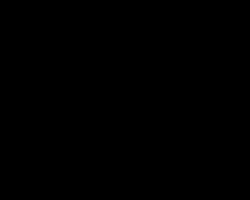
\includegraphics[scale=0.4]{BlobAnalysis/img/memory_0_0}} &
  50000 & 
  6250 & 
  0 \\
  \raisebox{1ex - \height}{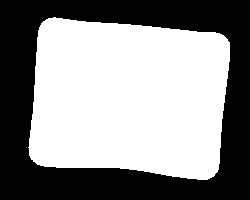
\includegraphics[scale=0.4]{BlobAnalysis/img/memory_1_163}} & 
  50000 & 
  6250 & 
  978 \\
  \raisebox{1ex - \height}{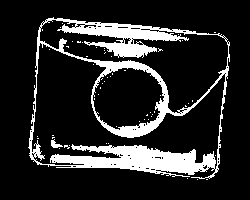
\includegraphics[scale=0.4]{BlobAnalysis/img/memory_2_1046}} & 
  50000 & 
  6250 & 
  6276 \\ 
  \raisebox{1ex - \height}{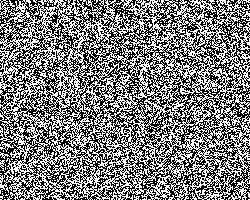
\includegraphics[scale=0.4]{BlobAnalysis/img/memory_3_12517}} & 
  50000 & 
  6250 & 
  75102  \\ 
\end{tabular}
\caption{Number of bytes consumed by different region representations.}
\label{tab:RegionRepresentationMemory}
\end{table}

\subsubsection{Region Dimensions}

\paragraph*{}
In our reference implementation, \studio, regions are represented using the run-length encoding described above, with one slight extension: each region stores two additional integers representing its reference dimensions: width and height.

\paragraph*{}
These are usually the dimensions of image the region was extracted from and serve two purposes. For one thing, they allow meaningful display of a region in the context of image it refers to; for other thing - they conveniently allow to define a complement of a region. Formally, the finite dimensions of the region space allows to distinguish between three types of pixels: set, unset and undefined (outside the region dimensions), i.e. corresponding to undefined image pixels that we have no information about.

\newarray\regionDimensions
\readarray{regionDimensions}{%
0 & 0 & 0 & 0 & 0 & 0 & 0 &%
0 & 1 & 1 & 1 & 0 & 0 & 0 &%
1 & 1 & 1 & 1 & 0 & 0 & 0 &%
0 & 0 & 1 & 0 & 0 & 0 & 0 &%
0 & 0 & 0 & 0 & 0 & 0 & 0}

\dataheight=\gridwidth

\begin{figure}[h!]
\centering

\begin{tikzpicture}[scale=0.40]\drawslabs{regionDimensions}\end{tikzpicture}
\caption{Region of dimensions: 7 (width), 5 (height)}
\label{tab:RegionDimensions}
\end{figure}